\documentclass[11pt,a4paper]{article}
\usepackage[a4paper,top=40mm,right=30mm,left=30mm,bottom=20mm]{geometry}
\usepackage[utf8]{inputenc}
\usepackage{amsmath}
\usepackage{amsfonts}
\usepackage{amssymb}
\usepackage{graphicx}
\author{Prakash Gautam}
\begin{document}
\begin{titlepage}
	\begin{center}
		\begin{Huge}
			Tribhuvan University\\
			
\includegraphics[scale=1.6]{./Images/logo.png}\\
			Institute of Engineering\\
			Pulchowk Campus\\[1.6cm]		
		\end{Huge}
		\textbf{A\\
		Mid Term Report On\\
		USB Oscilloscope Project}\\[1cm]
		\textbf{Submitted To:}\\
		Department of\\
		Electronics and Computer\\Engineering\\[1.6cm]
	
		\textbf{Submitted By:}\\
		Prajjwal Raj Kandel (068BEX428)\\
		Prakash Gautam (068Bex429)\\
		Sudip Prasai (068BEX442)\\
		Utsav Bhetwal (068BEX447)\\[1.5cm]
		\today	
	\end{center}
\end{titlepage}
\pagenumbering{roman}
\tableofcontents
\newpage
\abstract{\Large This is the Mid term report of out Project USB Oscilloscope. This briefly describes the progress made so far in the project and the works remaining. Since our primary goal is to show the waveform of the input analog signal, we have so far converted the analog value into digital value and have, at the moment, displayed in seven segment display. \\

The software interface required to display the graph of waveform has been completed and what remains is just communication between our system and the PC. After we send data back and forth from PC and the system we would be able to read the digital value of the input signal in the PC and display them as a function of time which is exaclty the waveform shown by the oscilloscope.\\
}


\newpage

\pagenumbering{arabic}

\section{Introduction}
One of the most frequent experiments students and researchers would do, working on study of electrical signals is to trace out the waveform of the signal as a function of time. This is done very successfully by a Oscilloscope. But the price that is attached with an Oscilloscope of a reasonable performance is beyond reach of many students. \\

In context of countries like Nepal, schools and colleges check their budget twice before even thinking of buying a new oscilloscope, let alone the curious students like us who can't even think of it.\\

But since computers have been vastly cheap and almost every student has a computer now, it makes sense to use the computational power of a computer to do the job of oscilloscope borrowing the help of computer screen to trace the electrical signals.\\

Our project is based upon the same idea of making oscilloscope assuming the availability of computer with relative ease than an oscilloscope. Furthermore parents would rather buy a multipurpose computer than an oscilloscope where they can't use Facebook on.\\

Additional small aid box beside that computer making it function as an oscilloscope would sound extremely great.\\

\section{Objectives}
As a part of syllabus of IOE, students of III${}^{rd}$ yr II${}^{nd}$ part are required to carry out a mini project. This project of ours is primarily intended for the fulfillment of the same. But we are committed to make this project not \emph{just another project}, we are expecting some real usefulness beside completing the requirement together with learning basic hardware electronics coupled with software interface.\\

We hope to learn a great deal of electronics on the application level.\\

Some of the objectives can be listed as:\\
\begin{enumerate}
	\item To fulfill the course requirement.
	\item To learn software and hardware integration on real scale
	\item To create easily affordable oscilloscope for students.
\end{enumerate}

\section{Hardware Selection}
Different hardware components used in the project are described in brief in the following section. Microcontroller is the primary hardware used and the major hardware is the display unit of computer.
\subsection{Microcontroller}
We have used ATMEGA16 as the Microcontroller. It has a built in ADC of 10bit resolution and can run at a clock frequency 16MHz which is sufficient for our requirement of the ADC conversion rate.

\begin{figure}[h]	
	\centering
	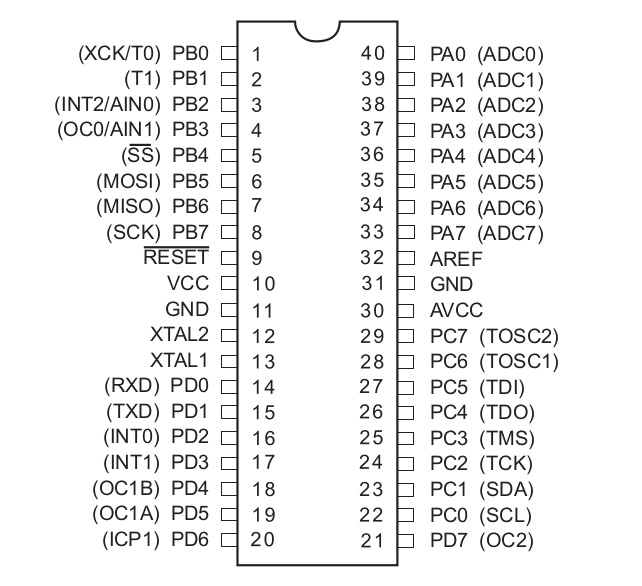
\includegraphics[scale=.35]{Images/Atmega16PinOut.png}
	\caption{Atmega16 Pinout}
	\label{fig:PinOut}
\end{figure}

Also it provides 16KB flash memory which is sufficient for our project.

\subsection{Programmer}
We have used USBasp programmer to upload program to the microcontroller. The programmer is made form ATMEGA8 microcontroller. We opted to get one already available in the market.
\begin{figure}[hbtp]
\centering
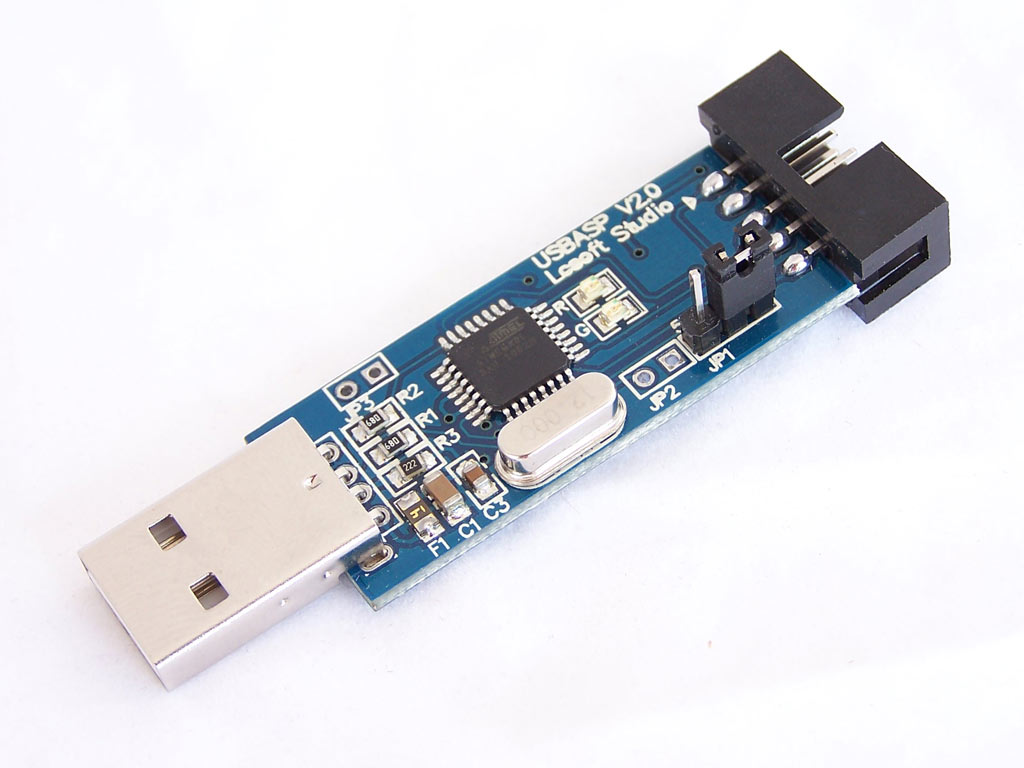
\includegraphics[scale=.18]{./Images/usbaspver2.jpg}
\caption{USBasp Programmer}
\end{figure}

\subsection{Voltage attenuator}
Since the input voltage of the Microcontroller is just 5V, and our oscilloscope needed to convert wider ranges of voltages into the range 0-5V, for this we needed voltage attenuator. We have decided to use instrumentation amplifier to regulate voltage to that level. The schematic circuit for the voltage attenuator is:
\begin{figure}[hbtp]
	\centering
	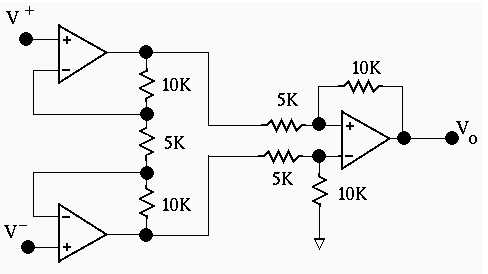
\includegraphics[scale=.4]{./Images/Amplifier.png}
	\caption{Instrumentation Amplifier}
\end{figure}

\newpage
\section{Softwares}
The software interfaces are made in C++ programming language and compiled for Linux Operating system. But the programms are made platform independent and can be easily compiled for other operating systems with just minor changes
\subsection{Graph Plotter}
We have made a graph plotter in C++ programming language with \textit{WxWidget 3.0.0} library. This plotter will be used to show the graphical representation of the waveform. The interface looks like,
\begin{figure}[hbtp]
	\centering
	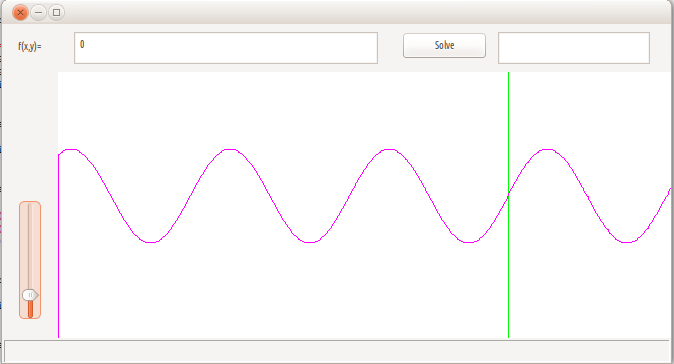
\includegraphics[scale=.6]{Images/Plotter.png}
	\caption{Graph Plotter}
\end{figure}


\subsection{Program Compiler and Uploader}	
We have even made our own programming software interface. This utilizes the \emph{avr-gcc} compiler and uses AVRDUDE to interface the programmer and the software interface. This can be used to upload program to various variants of atmega microcontroller.\\

\begin{figure}[hbtp]
\centering
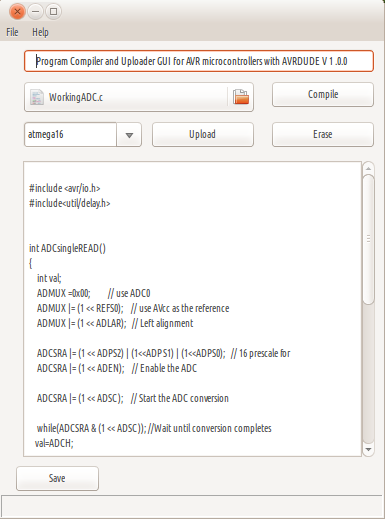
\includegraphics[scale=.4]{Images/AvrGUI.png}
\caption{Programmer Software Interface}
\end{figure}

This too is made in C++ programming language with wxWidget and can easily be extended to write program for other microcontrollers too. 

\section{Circuit Schematics}
So far we have interfaced adc and have successfully converted analog voltage into digital value and have scaled the digital output in the range of 0-9. So 5v input will be displayed in 7 segment as 9 and 0v will be shown 0 and 2.5v will correspond to 4. 
\begin{figure}[hbtp]
	\centering
	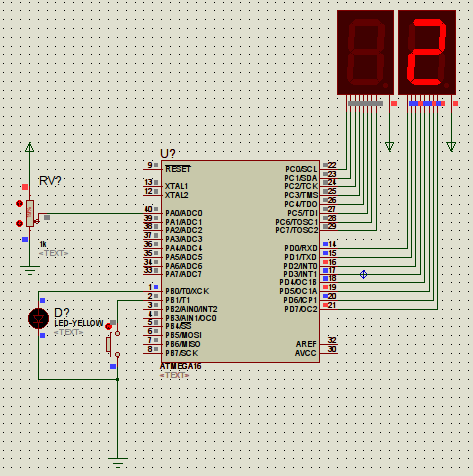
\includegraphics[scale=.5]{Images/Circuit.png}
	\caption{Cricuit So Far}
\end{figure}
\newpage

\section{Budget}
The costs of the major components required for this project are listed in the table below. And by the looks of it, the cost of this oscilloscope is going to become very much within reach of a normal student, which is our prime objective.
\begin{table}[h]
	\centering
	\begin{tabular}{c c c}
	\textbf{Component Name}  & \textbf{Unit} & \textbf{Cost} \\ 
	\hline
	Atmega16 & 1 & 400 \\ 
	Programmer & 1 & 1200 \\ 	 
	7 Segment Display & 4 & 100 \\ 
	7805 & 1 & 15 \\  
	Potentiometer & 1 & 10 \\  
	Total & {} & 1725 \\
	\end{tabular} 
	\caption{Component Cost}
\end{table}
\section{Conclusion}
We are very much confident that we can complete the project in time. This project, though not completed yet, has taught us a lot of things on micro-controller programming. Though only the beginning of micro-controller programming, this project has made us pretty excited on building some hardware architecture. Beginning with almost zero knowledge on micro-controller based hardware, this project has made us go through so many e-books and video tutorials. Therefore, we have helped ourselves with self learning and some sort of combined study with the project members.


Though we do not have any hard and fast schedule for accomplishing the project, for the time being we are ahead of what could have been an ideal schedule for this project. The solutions of the problems are being dealt with pretty effectively and we are more than confident that this project will be completed in time.
Apart from the things we learn through this project, we believe this project can also become a quite applicable one in modern day technology. 

\begin{thebibliography}{99}
\bibitem{} Alexon, J. USB Complete: The Developer’s Guide, Fourth Edition. Lakeview Research LLC, 5310 Chinook Ln., Madison  (1999).

\bibitem{} Wikipedia the open internet library \emph{http://en.wikipedia.org/Oscilloscope}
\bibitem{} \emph{codeandlife.com/VUsb}

\end{thebibliography}
\end{document}